\chapter{Generatívne systémy}

Doteraz sme sa zaoberali iba paralelnými modelmi, ktorých
spoločnou črtou bola akási\linebreak ``gramatiková filozofia'',
teda mali sme množinu symbolov, počiatočný symbol, resp.
počiatočné slovo a akúsi množinu prepisovacích pravidiel, ktoré
striktne riadili odvodenie a celý mechanizmus generoval nejaký
jazyk. Ukážeme si trošku iný pohľad na vec, nový z hľadiska
spôsobu prepisovania, kedy zostane zachovaná ``viditeľná
gramatiková časť'', teda symboly, počiatočný symbol, zmení sa však
prepisovací mechanizmus. Ako uvidíme neskôr, pôjde o akúsi
kombináciu gramatikového a automatového pohľadu na jazyky. Pomocou
tohto mechanizmu bude možné simulovať už známe gramatiky, či už z
Chomského hierarchie, alebo skôr spomenuté paralelné gramatiky.
Zaujímavý (a veľmi dôležitý) na tomto modeli je fakt, že pomerne
jednoducho umožní porovnať paralelné a sekvenčné formalizmy z
hľadiska zložitosti, a tým ukázať, v ktorej oblasti nám
paralelizmus pomôže a kde naopak nemá zmysel sa ním veľmi
zaoberať.

\section{Definície a označenia}

\begin{definicia}
Abstraktný generatívny systém je štvorica $G=(N,T,f,\sigma)$ kde
$N$ je množina neterminálov, $T$ je množina terminálov, $f$ je
konečne zadaná funkcia $(N\cup T)^* \ra 2^{(N\cup T)^* }$,
$\sigma$ je počiatočný neterminál pričom $N,T$ nie sú nutne
disjunktné abecedy.
\end{definicia}

\begin{definicia}
Krok odvodenia abstraktného generatívneho sytému je relácia $\Ra$
na $(N\cup T)^* $ definovaná takto: $u\Ra v$ práve vtedy keď $v\in
f(u)$.
\end{definicia}

\begin{definicia}
Jazyk generovaný abstraktným generatívnym systémom $G$ je množina
$L(G)$, pričom \mbox{$L(G)=\{w\in T^* \mm\sigma\overset{* }\Ra
w\}$}.
\end{definicia}

V ďalšom sa budeme zaoberať špeciálnym typom abstraktných
generatívnych systémov, a to generatívnymi systémami.

\begin{definicia}
1-$a$-prekladač je $a$-prekladač
$M=(K,\Sigma_1,\Sigma_2,H,q_0,F)$, v ktorom množina štvoríc je
tvaru\footnote{1-$a$-prekladač nemá pružnú čítaciu hlavu t.j. môže
čítať práve jeden symbol} $H\subseteq K\times\Sigma_1\times
{\Sigma_2}^* \times K$.
\end{definicia}

\begin{definicia}
Generatívny systém ($g$-systém) je abstraktný generatívny systém,
v ktorom $f$ je zobrazenie 1-$a$-prekladačom. Zapisujeme
$G=(N,T,M,\sigma)$ kde $M$ je 1-$a$-prekladač.
\end{definicia}

\begin{definicia}
Krok odvodenia $g$-systému je relácia $\Ra$ na $(N\cup T)^* $
definovaná takto: $u\Ra v$ práve vtedy\footnote{pre vstupné slovo
$u$ 1-$a$-prekladač $M$ vygeneruje výstup $v$} keď $v\in M(u)$.
\end{definicia}

\begin{priklad}
\label{gs_prikl_aprekladac} Zostrojíme $g$-systém  $G=(N,T,M,S)$ pre jazyk
$L=\{ww\mm w\in\{a,b\}^*\}$. Neterminály budú $N=\{S,A\}$,
terminály $T=\{a,b\}$, $a$-prekladač $M$ bude (obr.\ref{fig:gsystem-priklad}).
\begin{figure}[!ht]
  \centering
  \includegraphics{img/gsystems/gsystem-priklad.1.mps}
  \caption{$a$-prekladač $g$-systému pre jazyk $L$ z príkladu
    \ref{gs_prikl_aprekladac}}
  \label{fig:gsystem-priklad}
\end{figure}
\end{priklad}

\begin{oznacenie}
$\mathcal{G}$  trieda všetkých $g$-systémov. \\
$\mathcal{G_\varepsilon}$ trieda všetkých bez-$\varepsilon$
$g$-systémov, t.j. 1-$a$-prekladač nedáva na výstup $\varepsilon$.
\end{oznacenie}

\section{Porovnanie generatívnej sily $g$-systémov s gramatikami Chomského hierarchie}

\begin{veta}
\label{gs_veta_gre} $\mathcal{L}_{\mathcal{G}}=\mathcal{L}_{RE}$
\end{veta}

\begin{dokaz}
Dokážeme obe inklúzie:
\begin{description}
\item{$\subseteq$:} Táto inklúzia vyplýva z Turingovej tézy, ale
iste by sme si vedeli predsaviť aj TS, ktorý dostane na pásku
slovo a na druhej páske simuluje odvodenie tohto slova
$g$-systémom od počiatočného neterminálu a porovnáva, či je slovo
z druhej pásky zhodné so vstupom na prvej páske.
\item{$\supseteq$:} Pomocou $g$-systémov chceme simulovať frázové gramatiky, t.j. ku každej
frázovej gramatike $G$ treba zostrojiť $g$-systém $G'$ taký, že
$L(G')=L(G)$. $G'$ zostrojíme nasledovne:\newline ku každému
pravidlu $a_1a_2\dots a_n\ra b_1b_2\dots b_m$ urobíme v
$g$-systéme cestu ako na\linebreak obrázku \ref{fig:re-to-gsystem}.
\end{description}
\end{dokaz}

\begin{figure}[!ht]
    \centering
    \includegraphics{img/gsystems/re-to-gsystem.1.mps}
    \caption{Konštrukcia $g$-systému ku frázovej gramatike}
    \label{fig:re-to-gsystem}
\end{figure}

\pagebreak

\begin{veta}
\label{gs_veta_gre2}
$\mathcal{L}_{\mathcal{G}_\varepsilon}=\mathcal{L}_{CS}$
\end{veta}

\begin{dokaz}
Dokážeme obe inklúzie:
\begin{description}
\item{$\subseteq$:} K bez-$\varepsilon$ $g$-systému zostrojíme LBA
akceptujúci ten istý jazyk. LBA si, rovnako ako TS\linebreak v
predchádzajúcej vete, vyrobí druhú pásku, na ktorej bude simulovať
odvodenie vstupného slova simulovaným $g$-systémom. Keďže
$g$-systém je bez $\varepsilon$, nemôže sa stať, že pri odvodení
nejakého slova $w$ vznikne vetná forma dĺžky väčšej ako je $|w|$.
Preto na simuláciu stačí priestor ohraničený dĺžkou vstupného
slova, a teda vystačíme s LBA.
\item{$\supseteq$:} Konštrukcia je podobná ako v predchádzajúcej vete
(obr.\ref{fig:cs-to-gsystem}) s využitím toho, že v kontextových gramatikách nie
je pravá strana pravidla kratšia ako ľavá, takže v konštrukcii
1-$a$-prekladača nepotrebujeme pravidlá s $\varepsilon$ výstupom.
\end{description}
\end{dokaz}

\begin{figure}
    \centering
    \includegraphics{img/gsystems/cs-to-gsystem.1.mps}
    \caption{Konštrukcia $g$-systému ku kontextovej gramatike}
    \label{fig:cs-to-gsystem}
\end{figure}

\begin{definicia}
Kopírovací cyklus v 1-$a$-prekladači je štvorica z $H$ tvaru
$(q,a,a,q)$.
\end{definicia}

\begin{definicia}
$g$-systém je sekvenčný, ak jediné cykly v 1-$a$-prekladači sú
kopírovacie cykly v počiatočnom alebo koncovom stave.
\end{definicia}

\begin{oznacenie}
$\mathcal{S}$ trieda všetkých sekvenčných $g$-systémov.\\
$\mathcal{S}_\varepsilon$ trieda všetkých bez-$\varepsilon$
sekvenčných $g$-systémov.
\end{oznacenie}

\pagebreak

\begin{veta}\label{gs_veta_gsek}
$\mathcal{L}_{\mathcal{S}}=\mathcal{L}_{RE},
\mathcal{L}_{\mathcal{S}_\varepsilon}=\mathcal{L}_{CS}$
\end{veta}

\begin{dokaz}
Konštrukcia je tá istá ako vo vete \ref{gs_veta_gre}, resp.
\ref{gs_veta_gre2}, lebo ľahko vidno, že zostrojený $g$-systém je
sekvenčný.
\end{dokaz}

\section{Modelovanie známych gramatík pomocou $g$-systémov}

\begin{priklad}
    Ukážeme si, že pomocou $g$-systémov vieme jednoducho modelovať
    $EOL$ a bezkontextové gramatiky:
    \begin{description}
    \item{$EOL$:} Nech množina pravidiel $EOL$ je
        $P=\{ a_1\pravidlo u_1,a_2\pravidlo u_2,\dots,a_n\pravidlo
        u_n\}$.
        Potom príslušný $g$-systém bude vyzerať ako na obrázku
        \ref{fig:eol-to-gsystem}a.

    \item{$CF$:} Nech množina pravidiel $CF$ je
        $P=\{a_1\pravidlo u_1, a_2\pravidlo u_2,\dots,a_n\pravidlo
        u_n\}$. Príslušný $g$-systém zostrojíme podľa obrázku
        \ref{fig:eol-to-gsystem}b.
    \end{description}

    \begin{figure}[!ht]
        \centering
        \subfigure[EOL]{
            \includegraphics{img/gsystems/eol-to-gsystem.1.mps}
        }
        \subfigure[CF]{
            \includegraphics{img/gsystems/cf-to-gsystem.1.mps}
        }
        \caption{Modelovanie $EOL$-systémov a
                    $CF$-gramatík pomocou $g$-systémov}
        \label{fig:eol-to-gsystem}
    \end{figure}
\end{priklad}

\begin{poznamka}
Gramatika $G$ je bezkontextová práve vtedy, keď existuje sekvenčný
$g$-systém $G'$ s dvoma stavmi taký, že $L(G)=L(G')$. Implikácia
``$\Ra$'' vyplýva z konštrukcie na\linebreak obrázku \ref{fig:eol-to-gsystem}b,
dôkaz opačnej implikácie nie je triviálny a presahuje rámec tohto
textu.
\end{poznamka}

\begin{veta}
Absolutne paralelné gramatiky sú ekvivalentné s $g$-systémami
spĺňajúce nasledujúce podmienky (ozn. $\tilde{\mathcal{G}}$ trieda
takýchto $g$-systémov):
\begin{enumerate}
  \item každý cyklus je kopírovací cyklus pre terminál
  \item v každom stave je kopírovací cyklus pre každé $a\in T$
  \item terminálne symboly sú prepisované len v kopírovacích cykloch
\end{enumerate}
\end{veta}

\begin{dokaz}
Máme dokázať, že
$\mathcal{L}_{AP}=\mathcal{L}_{\tilde{\mathcal{G}}}$
\begin{description}
\item{$\subseteq$:} K danej $AP$ gramatike $G$ zkonštruujeme ekvivalentný $g$-systém
$G'\in\tilde{\mathcal{G}}$ nasledovne. Každému pravidlu v $G$
tvaru $(A_1,\dots A_k)\ra (w_1,\dots w_k))$ zodpovedá v
1-$a$-prekladači $g$-systému $G'$ práve jedna cesta znázornená na
obrázku \ref{fig:ap-to-gsystem}.

\begin{figure}[!ht]
    \centering
    \includegraphics{img/gsystems/ap-to-gsystem.1.mps}
    \caption{Konštrukcia $g$-systému k $AP$ gramatike}
    \label{fig:ap-to-gsystem}
\end{figure}

\item{$\supseteq$:} Pre každú cestu v 1-$a$-prekladači z $q_0$ do $q_F$
(mimo kopírovacích cyklov) v $AP$ gramatike urobíme pravidlo:
$(A_1,\dots A_k)\ra (w_1,\dots w_k))$.
\end{description}
\end{dokaz}

\section{Miery zložitosti}

\begin{itemize}
\item $STATE(G)=$ počet stavov 1-$a$-prekladača $g$-systému $G$
\item $ARC(G)=$ počet pravidiel 1-$a$-prekladača $g$-systému $G$
\item $STATE_U(L)=\min\{ STATE(G)\mm L=L(G), G\in U\}$
\item $ARC_U(L)=\min\{ ARC(G)\mm L=L(G), G\in U\}$
\item $TIME(G,w)=\min\{ k\mm\sigma\overset{k}{\underset{G}{\Ra}} w\}; w\in L(G)$
\item $TIME(G,n)=\max\{ TIME(G,w)\mm w\in L(G), |w|\leq n\}$
\item $TIME_U(f(n))=\{ L \mm \exists G\in U, L=L(G), TIME(G,n)=O(f(n))\}$
\item $\overline{TIME}_U(f(n))=\{ L\mm\forall G\in U, L=L(G), TIME(G,n)=\Omega(f(n))\}$
\item $SPACE(G,w)=\min\{ SPACE(\alpha )\}$; kde $\alpha$ : $\sigma\Ra u_1\Ra\dots\Ra u_n$ je odvodenie $w$ v $G$
a $SPACE(\alpha)=\max\{|u_i|\mm 0\leq i\leq n\}$
\end{itemize}

\begin{veta}
Pre každý nekonečný jazyk $L$ platí:
\begin{enumerate}
\item $L\in\overline{TIME}_{\mathcal{S}}(n)$
\item $L\in\overline{TIME}_{\mathcal{G}}(\log n)$
\end{enumerate}
\end{veta}

\begin{dokaz}
\begin{enumerate}
\item Nech $G\in\mathcal{S}$. Zamyslime sa nad tým, aké najdlhšie
slovo môže vygenerovať $G$ na $n$ krokov. $G$ dokáže v jednom
kroku prepisovať len jeden súvislý úsek vetnej formy. Túto vetnú
formu dokáže $G$ predĺžiť o najviac

\centerline{$m=\max\{$ súčet dĺžok výstupov na jednej ceste v
1-$a$-prekladači - dĺžka tejto cesty $\}$} Majme odvodenie $\sigma
=w_0\Ra w_1\Ra\dots\Ra w_i\Ra w_{i+1}\Ra\dots\Ra w_n$. Potom
platí\linebreak $|w_{i+1}|\leq |w_i| + m$. Keďže $|w_0|=|\sigma
|=1$, tak $|w_n|\leq 1 + nm$. Z toho teda nakoniec plynie, že $G$
potrebuje na vygenerovanie slova dĺžky $n$ aspoň lineárny čas.
\item Nech $G\in\mathcal{G}$. $G$ môže v každej vetnej forme
prepísať všetky symboly. Označme

\centerline{$m=\max\{$ výstup v 1-$a$-prekladači $\}$} Potom platí
$|w_{i+1}|\leq |w_i|.m$. Keďže $|w_0|=|\sigma |=1$, tak $|w_n|\leq
m^n$. Z toho plynie, že $G$ potrebuje na vygenerovanie slova dĺžky
$n$ aspoň logaritmický čas
\end{enumerate}
\end{dokaz}

\section{Porovnanie sekvenčných a paralelných $g$-systémov}
\label{gs_sec_sekvspar}

\begin{veta}
\label{gs_veta_parsek}
$\mathcal{L_G=L_S,L_{G_{\varepsilon}}=L_{S_{\varepsilon}}}$
\end{veta}

\begin{dokaz}
Tvrdenie priamo vyplýva z viet \ref{gs_veta_gre}, \ref{gs_veta_gre2} a
\ref{gs_veta_gsek} a hovorí nám, že paralelné a sekvenčné $g$-systémy
sú z hľadiska generatívnej sily ekvivalentné, no nedáva nám žiadny
návod, ako ku paralelnému $g$-systému nájsť sekvenčný, rovnako nič
nehovorí o tom, aký vplyv bude mať táto konštrukcia na popisnú
zložitosť.

Ukážeme si, ako k ľubovoľnému $g$-systému $G\in\mathcal{G}$
zkonštruujeme $g$-systém $G''\in\mathcal{S}$ \mbox{s ním}
ekvivalentný (t.j. $L(G)=L(G'')$) a potom si povieme, ako sa
``zosekvenčnenie'' odrazí na zložitosti.

Nech $G=(N,T,M,\sigma)$ je ľubovoľný $g$-systém,
$L(G)\in\mathcal{L_G}$, počiatočný stav $M$ je $q_0$ a koncový
$q_F$. Uvedomme si, čo potrebujeme na $G$ prepracovať, aby sme ho
``zosekvenčnili''. \mbox{V prvom} rade potrebujeme mať v
po\-čia\-toč\-nom aj koncovom stave kopírovacie cykly pre
všetky\footnote{ako sa neskôr ukáže, tak nie nutne pre úplne
všetky, stačí pre niektoré} symboly, aby sme sa vo vetnej forme
mohli presunúť ľubovoľne ďaleko, potom niečo $a$-prek\-la\-da\-čom
prepísať a vetnú formu dokopírovať do konca. V druhom rade
potrebujeme odstrániť \mbox{z $G$} vnútorné cykly (teda všetky
také, ktoré nie sú kopírovacími cyklami v počiatočnom,
\mbox{resp.} koncovom stave). Keď sa nám toto podarí, budeme s
konštrukciou hotoví. $G''$ budeme konštruovať v dvoch krokoch:
\begin{enumerate}
  \item Zostrojíme $G'=(N',T,M',\underline{\overline{\sigma}})$
  ekvivalentný s $G$ s užitočnými technickými vlastnosťami, ktoré
  neskôr využijeme:
  \begin{enumerate}
    \item zavedieme nový počiatočný stav $q_0'$ a nový koncový stav
    $q_F'$ a v týchto stavoch zkonštruujeme kopírovacie
    cykly\footnote{Zrejme by nestačilo dodať kopírovacie cykly do
    $q_0$, resp. $q_F$. Mohlo by sa totiž ľahko stať, že by sme takto
    zkonštruovaným 1-$a$-prekladačom akceptovali aj to, čo
    1-$a$-prekladač v $G$ neakceptoval} $\forall a\in(N'\cup T)$, $N'$
    definujeme neskôr, označme množinu týchto kopírovacích cyklov
    $C=\{(q,a,a,q)\mm q\in\{q'_0,q'_F\},a\in(N\cup T)\}$.
    \item $G'$ bude udržovať informáciu o prvom  a poslednom symbole
    vetnej formy tak, že ich označí: prvý symbol horným prúžkom,
    posledný dolným prúžkom. Označené symboly budú nové neterminály, v
    $G'$ musíme vytvoriť nové podčiarknuté aj nadčiarknuté symboly,
    teda $N'=N\cup\{\overline{a}\mm a\in(N\cup T
    )\}\cup\{\underline{a}\mm a\in(N\cup
    T)\}\cup\{\underline{\overline{\sigma}}\}$. Počiatočný neterminál
    $G'$ bude $\underline{\overline{\sigma}}$. Vetná forma bude
    vyzerať nasledovne: $\overline{a}_1 a_2 a_3\dots
    a_{n-1}\underline{a_n}$.
  \end{enumerate}
  Teraz poďme konštruovať $G'$ tak, aby sme zabezpečili obe
  ``dobré'' vlastnosti, ktoré sme uviedli a zároveň aby boli $G$ a
  $G'$ ekvivalentné. Zrejme bude potrebné upraviť prechodovú množinu
  1-$a$-prekladača. Ak $H$ bola prechodová množina $M$, tak $H_{M'}$
  bude prechodová množina $M'$. Zatiaľ definujme $H'$ nasledovne
  (nech $a,d,A,B\in(N\cup T),b,c\in(N\cup T)^*$):
  \[
  H'=H\cup C\cup\{(q'_0,\overline{A},\overline{a}b,q_1)\mm
  (q_0,A,ab,q_1)\in H\}\cup \{(q,\underline{B},c
  \underline{d},q'_F)\mm(q,B,cd,q_F)\in H\}
  \]
  Ak sa nad $H'$ trochu zamyslíme, tak je jasné, že v $q'_0$, resp.
  v $q'_F$ síce máme kopírovacie cykly, ale nebudeme ich používať.
  Keby sme totiž použili ľubovoľný kopírovací cyklus v $q'_0$, tak
  sa už z tohto stavu nikdy nedostaneme, pretože z neho vedú iba
  šípky na nadčiarknutý, teda prvý, symbol vetnej formy. Čo sa týka
  stavu $q'_F$, tak do neho sa možno dostať iba na podčiarknutý,
  teda posledný, symbol vetnej formy.

  Aby sme našu konštrukciu príliš nepretechnizovali, nebudeme sa
  zaoberať detailami oh\-ľa\-dom počiatočného neterminálu
  $\underline{\overline{\sigma}}$ a vynecháme aj prípady, kedy $M$
  ``príliš veľa'' vymazáva, teda ak sa v odvodení môže vyskytnúť
  vetná forma obsahujúca jediný symbol, prípadne $\varepsilon$.
  Pozrime sa teraz na $g$-systém, ktorý sme zkonštruovali. Keby sme
  uvažovali $G\in\mathcal{G_{\varepsilon}}$, tak už teraz máme (až
  na prvý a posledný symbol, s ktorým budeme pracovať neskôr) $G'$
  ekvivalentný s $G$ a splnené (a) aj (b). Ale my uvažujeme
  $G\in\mathcal{G}$. Uvedomme si, aké nepríjemnosti nám môže
  spôsobiť skutočnosť, že 1-$a$-prekladač môže zapisovať na výstup
  $\varepsilon$. Môže sa stať, že v $H$ existuje
  $(q_0,A,\varepsilon,q_1)$. Podľa doterajšej konštrukcie by sme do
  $H'$ pridali $(q'_0,\overline{A},\varepsilon,q_1)$. Tým by sme ale
  vymazali prvý symbol vetnej formy a 1-$a$-prekladač by nepracoval
  v ďaľších krokoch odvodenia správne. Podobne sa nám môže stať,
  že\linebreak v $H$ existuje $(q,B,\varepsilon,q_F)$, potom by sme
  do $H'$ pridali $(q,\underline{B},\varepsilon,q'_F)$, teda by sme
  si zmazali posledný (podčiarknutý) symbol vetnej formy a v ďaľšom
  kroku odvodenia by nastali problémy s akceptovaním. Ukazuje sa
  teda, že predchádzajúcu konštrukciu možno použiť iba na tie
  $(q,a,u,p)$, kde $u\neq\varepsilon$ (zámerne sme do tretej
  komponenty vždy písali reťazec $w\in(N'\cup T)^+$).

  Pre $\varepsilon$-výstupy 1-$a$-prekladača použijeme nasledovnú
  konštrukciu:
  \begin{enumerate}
    \item 1-$a$-prekladaču $M'$ pridáme nové stavy tak, že pre každý
    stav $q$ 1-$a$-prekladača $M$ vyrobíme nový stav $\overline{q}$. V
    týchto stavoch si budeme pamätať, že sme si zmazali prvý symbol
    vetnej formy a keď budeme robiť v danom kroku odvodenia prvý
    ne-$\varepsilon$ výs\-tup, tak prvý symbol z neho bude zároveň aj
    prvým symbolom vetnej formy, a tak mu pridáme čiaru hore. Teraz to
    všetko formálne zapíšeme. Označme $\overline{H}$prechodovú
    množinu, ktorú definujeme nasledovne ($a,b\in (N\cup T)$, $u\in(N\cup T)^*$):
    \begin{tabbing}
      \= xx \= $H$ \= $=$ \= xxxxxxxxxxxxxxxxxxxxxxxxxxxxxxxx \= \kill
      \>\>$\overline{H}$\>$=$\>
      $\{(q'_0,\overline{A},\varepsilon,\overline{q}_1)\mm
      (q_0,A,\varepsilon,q_1)\in H\}\med\cup$\>pamätáme si, že sme
      zmazali $\overline{A}$
      \\ \>\>\>$\cup$\>$\{(\overline{q},a,\varepsilon,\overline{p})\mm
      (q,a,\varepsilon,p)\in H\}\med\cup$\>stále sme nezapísali prvý
      symbol \\ \>\>\>$\cup$\>$\{(\overline{q},a,\overline{b}u,p)\mm
      (q,a,bu,p)\in H\}$\>zapíšeme $\overline{b}u$
    \end{tabbing}
    \item 1-$a$-prekladaču $M'$ pridáme nové stavy tak, že pre každý
    stav $q$ 1-$a$-prekladača $M$\linebreak vyrobíme nový stav $\underline{q}$.
    Tieto stavy budeme používať na to, aby sme si nezmazali posledný
    (podčiarknutý) symbol vetnej formy. Tu to však nebude také
    jedno\-znač\-né ako pri prvom symbole. Pretože 1-$a$-prekladač sa
    nemôže vracať, tak po tom, ako zmaže posledný symbol, už nemôže
    označiť čiarou dole nejaký iný. Na to, že raz zmaže posledný
    symbol vetnej formy, musí prísť ``dostatočne skoro'', využijeme
    možnosť nedeterminizmu. Uhádneme, že istý symbol vo vetnej forme
    je posledný, ktorý reálne zapisujeme, \mbox{a že} to, čo vznikne
    prepísaním symbolov za ním budú iba $\varepsilon$, a potom len
    kontrolujeme, či sme hádali správne. Formálne zapísané v
    prechodovej množine $\underline{H}$ ($w\in(N\cup T)^*$):
    \begin{tabbing}
      \= xx \= $H$ \= $=$ \= xxxxxxxxxxxxxxxxxxxxxxxxxxxxxx \= \kill
      \>\>$\underline{H}$\>$=$\>
      $\{(q,a,w\underline{b},\underline{p})\mm (q,a,wb,p)\in
      H\}\med\cup$\>nedet. zapíše nový posledný symbol\\
      \>\>\>$\cup$\>$\{(\underline{q},a,\varepsilon,\underline{p})\mm
      (q,a,\varepsilon,p)\in H\}\med\cup$\>stále maže všetky symboly\\
      \>\>\>$\cup$\>$\{(\underline{q},\underline{a},\varepsilon,q'_F)\mm
      (q,a,\varepsilon,q_F)\in H\}$\>ak zmaže posledný symbol, akceptuje
    \end{tabbing}
    Vytvorili sme akoby virtuálne $g$-systémy
    $G,\underline{G},\overline{G}$ (obr.\ref{gs_obr_gsp1}), pričom v
    jednom kroku odvodenia sa môžeme medzi nimi pohybovať. Neexistujú
    však žiadne šípky $G\ra\overline{G}$, $\underline{G}\ra
    G$, $\underline{G}\ra\overline{G}$.

    \begin{figure}[!ht]
      \centering
      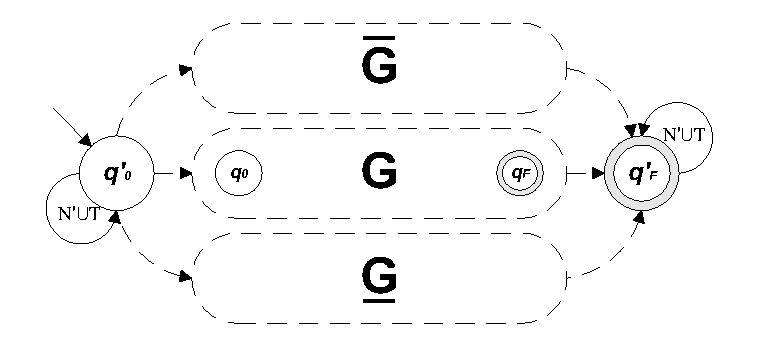
\includegraphics{img/gsystems/g_s_p_1}
      \caption{1-$a$-prekladač $g$-systému $G'$} \label{gs_obr_gsp1}
    \end{figure}

    Na to, aby sme mali $L(G)=L(G')$ ešte potrebujeme v istom kroku
    odznačiť prvý aj posledný označený symbol. Avšak keďže máme v
    1-$a$-prekladači $g$-systému $G'$ šípky z $q'_0$ do iného stavu,
    resp. šípky do $q'_F$ z iného stavu (teda nie kopírovacie cykly v
    týchto stavoch) iba na označený symbol, tak s odznačenou vetnou
    formou už ďalej nepohneme. Z toho plynie, že symboly možno
    odznačiť len v poslednom kroku odvodenia, teda vtedy, ak všetky
    symboly vetnej formy, okrem prvého a posledného, sú terminály a aj
    prvý a posledný symbol (odhliadnuc od označenia) sú terminály.
    Teda opäť nedeterministicky hádame posledný krok. Formálne
    definujme:
    \[
    H_T=\{(q'_0,\overline{a},a,q_T),(q_T,a,a,q_T),
    (q_T,\underline{a},a,q'_F)\mm a\in T\}
    \]
    $q_T$ je nový stav 1-$a$-prekladača $g$-systému $G'$. Zachovali
    sme konzistentnosť v tom zmysle, že z $q'_0$ vychádzajú, okrem
    kopírovacích cyklov, iba šípky na prvý (nad\-čiar\-knu\-tý) symbol
    a do $q'_F$ vchádzajú, okrem kopírovacích cyklov, iba šípky na
    posledný\linebreak (pod\-čiar\-knu\-tý) symbol vetnej formy, teda máme
    $L(G)=L(G')$, pričom\newline $G'=(N',T,M',\underline{\overline{\sigma}})$.
    Čo sa týka $M'$ pre nás je zaujímavé, ako sa zmenila prechodová
    množina: keď v $M$ to bola $H$, tak v $M'$ to bude
    $H_{M'}=H'\cup\overline{H}\cup\underline{H}\cup H_T$. Pokiaľ ide o
    stavy a abecedy, ich konštrukcia by mala byť z už uvedeného
    zrejmá.
  \end{enumerate}
  \item Ku $G'=(N',T,M',\underline{\overline{\sigma}})$
  zostrojíme ekvivalentný $g$-systém $G''$ tak, že prerušíme všetky vnútorné cykly
  (teda tie, ktoré nie sú kopírovacie v počiatočnom alebo koncovom
  stave). Vonkajšou šípkou 1-$a$-prekladača nazveme takú, ktorá buď
  vychádza z počiatočného stavu, alebo vchádza do akceptačného stavu
  (v našom prípade ide o stavy $q'_0,q'_F$). Ostatné šípky nazveme
  vnútorné. Pri odstraňovaní cyklov budeme postupovať nasledovne:
  \begin{enumerate}
    \item stavy budú rovnaké ako v $G'$
    \item všetky vonkajšie šípky necháme tak ako sú
    \item každú vnútornú šípku nahradíme dvoma novými nasledovne: ak
    $(q,a,u,p)\in H_{M'}$, tak $(q,a,u,p)\not\in H_{M''},
    (q,a,[q,a,u,p],q'_{F})\in H_{M''}, (q'_0,[q,a,u,p],u,p)\in
    H_{M''}$, pričom $[q,a,u,p]$ budú nové neterminály\footnote{Ak sa
    čitateľ trochu zamyslí, malo by mu byť jasné, že v každom kroku
    môže byť vo vetnej forme najviac jeden takýto neterminál}
    (obr.\ref{gs_obr_gps2})
  \end{enumerate}

  \begin{figure}[!ht]
    \centering
    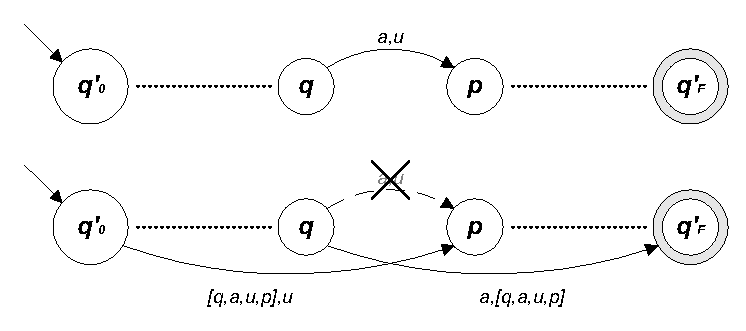
\includegraphics{img/gsystems/g_s_p_2}
    \caption{Nahrádzanie vnútorných šípok v $G''$} \label{gs_obr_gps2}
  \end{figure}

  Môže sa naskytnúť otázka: prečo sme nenahradzovali aj vonkajšie
  šípky? Odpoveď je veľmi jednoduchá: pretože ony žiadne cykly
  vytvárať nemohli, tak sme $G'$ konštruovali. Malo by byť zrejmé,
  že takto sme odstránili všetky cykly, okrem kopírovacích v
  počiatočnom a koncovom stave, lebo teraz všetky šípky vychádzajú z
  $q'_0$ alebo vchádzajú do $q'_F$ a toto sú jediné šípky v $G''$.
  Rovnako zrejmé by malo byť $L(G')=L(G'')$, v $G''$ sme iba
  nahradili jeden paralelný krok $n$ sekvenčnými, kde $n$ je počet
  šípok v jednom paralelnom kroku.
\end{enumerate}
Máme zkonštruovaný $g$-systém $G''$ taký, že $L(G)=L(G'')$ a
$G''\in\mathcal{S}$, teda naše ``zosekvenčňovanie'' $g$-systému
$G$ je na konci.
\end{dokaz}

Nasledujúce tvrdenia hovoria niečo o zložitosti $g$-systému ktorý
sme práve zostrojili v pred\-chá\-dza\-jú\-cej konštrukcii a
priamo z nej vyplývajú.

\begin{veta}
(Vzťah popisnej zložitosti sekvenčných a paralelných $g$-systémov)
\begin{itemize}
  \item $\forall L\med STATE_{\mathcal{S}}(L)\leq
  3.STATE_{\mathcal{G}}(L)+3$
  \item $ARC_{\mathcal{S}}(L)\leq 32.STATE_{\mathcal{G}}(L)+22.\#\Sigma_L$
\end{itemize}
\end{veta}

Je dobré si uvedomiť, že zosekvenčnením $g$-systému sme nepoužili
žiadny priestor navyše, o čom hovorí nasledujúca veta.

\begin{veta}
$SPACE_{\mathcal{S}}(f(n))=SPACE_{\mathcal{G}}(f(n))$ pre $\forall
f(n)$
\end{veta}

\begin{veta}\label{gs_veta_h_odhad}
Pre ľubovoľný jazyk $L$ a ľubovoľný
$G\in\mathcal{G}$ taký, že $L=L(G)$ platí:
\[
L\in
TIME_{\mathcal{S}}(SPACE_{\mathcal{G}}(G,n).TIME_{\mathcal{G}}(G,n))
\]
\end{veta}

Veta \ref{gs_veta_h_odhad} hovorí o akomsi hornom odhade počtu  krokov
sekvenčných \mbox{$g$-sys}té\-mov v porovnaní\linebreak s
paralelnými. Na bližšie pochopenie tohto tvrdenia si stačí
uvedomiť, že sekvenčný $g$-systém môže v jednom kroku vďaka tomu,
že nemá vnútorné cykly, prepísať len istý, vo všeobecnosti malý,
úsek vetnej formy na rozdiel od paralelného $g$-systému, ktorý
môže v jednom kroku prepísať celú vetnú formu. Teda ak chce
sekvenčný $g$-systém odsimulovať jeden krok paralelného\linebreak
$g$-systému, musí urobiť $\{$ rádovo dĺžka vetnej formy $\}$
krokov. Ak chceme sekvenčne odsimulovať celý výpočet paralelného
$g$-systému, dostávame spomínané tvrdenie.

\smallskip
Keď sa na tento problém pozrieme z opačnej strany (keď chceme
jazyk generovaný sekvenčným $g$-systémom, generovať paralelným
$g$-systémom), podobná úvaha nám umožňuje pretransformovať dolný
odhad počtu krokov pre sekvenčné $g$-systémy na dolný odhad počtu
krokov pre paralelné $g$-systémy. Dostávame teda nasledujúce
tvrdenie.

\begin{veta}
\label{gs_veta_d_odhad}
$\overline{TIME}_{\mathcal{S_{\varepsilon}}}(f(n))\subseteq
\overline{TIME}_{\mathcal{G_{\varepsilon}}}(\frac{f(n)}{n})$
\end{veta}

Toto tvrdenie nám ukazuje, že vzťah paralelných a sekvenčných
$g$-systémov je lineárny a teda, že paralelizmus nám vo
všeobecnosti veľmi nepomôže (aspoň nie nejak dramaticky), ako si
však neskôr ukážeme, existujú tzv. ``rýchlo generovateľné''
jazyky, kde je rozdiel výraznejší.

\begin{priklad}
Je známe, že $L=\{wcw\mm
w\in\{a,b\}^*\}\in\overline{TIME}_{\mathcal{S_{\varepsilon}}}(n^2)$,
teda podľa vety \ref{gs_veta_d_odhad} $L\in
TIME_{\mathcal{G_{\varepsilon}}}(n)$. Paralelizmus teda tomuto
jazyku veľmi nepomôže, nie je totiž exponenciálny
\end{priklad}

\section{Normálové tvary $g$-systémov}

\begin{definicia}
Hovoríme, že $g$-systém je v normálovom tvare, ak spĺňa
nasledujúce podmienky:
\begin{enumerate}
\item existuje kopírovací cyklus pre $\forall a\in N\cup T$ v $q_0$ aj v $q_F$
\item iba kopírovacie cykly vstupujú do $q_0$ a vystupujú z $q_F$
\item terminálne symboly sa iba kopírujú
\item $g$-systém je bez $\varepsilon$
\end{enumerate}
\end{definicia}

\begin{oznacenie}
$\mathcal{N}$ je trieda všetkých $g$-systémov v normálnom tvare
\end{oznacenie}

\begin{veta}
$\mathcal{L}_{\mathcal{N}}=\mathcal{L}_{\mathcal{G}_{\varepsilon}}$
\end{veta}

\begin{dokaz}
Inklúzia $\subseteq$ je zrejmá vďaka štvrtej podmienke. Dokážeme
opačnú inklúziu: \\ Nech
$G=(N,T,M,\sigma)\in\mathcal{G}_\varepsilon$. Chceme zostrojiť
$G''\in\mathcal{N}$ taký, že $L(G'')=L(G)$, teda chceme. aby $G''$
spĺňal všetky štyri podmienky z definície $\mathcal{N}$. Keďže
$G\in\mathcal{G}_\varepsilon$ tak podmienka 4 je automaticky
splnená. $G''$ zostrojíme v dvoch krokoch:
\begin{enumerate}
  \item Najskôr zostrojíme $G'=(N',T,M',\sigma)$ taký, že $L(G')=L(G)$ a $G'$ bude
  spĺňať tretiu podmienku z definície $\mathcal{N}$:
  \begin{itemize}
    \item $N'=N\cup\{\xi_a\mm a\in T\}$
    \item $\forall a\in T$ : všetky výskyty
    terminálu $a$ v $H$ nahradíme novým neterminálom $\xi_a$
    \item v $q_0$ nedeterministicky uhádneme, že vetná forma
    obsahuje už len neterminály typu $\xi_a$ a celú ju
    zterminálnime. Do $M'$ pridáme nový stav $q'$ a do $H'$
    pridáme štvorice: pre $\forall\; a\in T$ $(q_0,\xi_a,a,q')$
    a $(q',\xi_a,a,q')$, pričom $q'$ bude akceptačným stavom.
  \end{itemize}
  \item Na $G'$ použijeme konštrukciu podobnú s prvou časťou
  konštrukcie z kapitoly \ref{gs_sec_sekvspar}, ktorá nám zabezpečí
  splnenie podmienok 1 a 2. Všimnime si, že keďže pracujeme s bez
  $\varepsilon$ $g$-sytémami, tak nemusíme strojnásobovať stavy, a
  teda vychádzajú aj lepšie odhady popisnej zložitosti.
\end{enumerate}
\end{dokaz}

\begin{dosledok}
Pre každý jazyk $L\in\mathcal{L}_{\mathcal{G}_{\varepsilon}}$
platí:
\begin{enumerate}
  \item $STATE_{\mathcal{N}}(L)\leq STATE_{\mathcal{G}_{\mathcal{\varepsilon}}}(L)+3$
  \item $ARC_{\mathcal{N}}(L)\leq 12.ARC_{\mathcal{G}_{\varepsilon}}(L)+14.\#\Sigma_L$
  \item $SPACE_{\mathcal{N}}(n)=SPACE_{\mathcal{G}_{\varepsilon}}(n)=\mathcal{L}_{CS}$
  \item $TIME_{\mathcal{N}}(f(n))=TIME_{\mathcal{G}_{\varepsilon}}(f(n))$
\end{enumerate}
\end{dosledok}

\begin{oznacenie}
$STATE_{\mathcal{N}}(n)=\{ L\mm\exists G\in\mathcal{N}, STATE(G)\leq n, L=L(G)\}$
\end{oznacenie}

\begin{veta}
$STATE_{\mathcal{N}}(n)$ je $\mathcal{AFL}$ pre\footnote{pre $n=1$ by boli problémy s
$h^{-1}$} $\forall n>1$
\end{veta}

\begin{oznacenie}
$\mathcal{N}_{i,j}$ - trieda všetkých sekvenčných $g$-systémov v
normálnom tvare, ktoré majú najviac $i$ stavov a najviac $j$
neterminálov, pričom sú dovolené $\varepsilon$ prechody v
1-$a$-prekladači.
\end{oznacenie}

\pagebreak

\begin{veta}
$\mathcal{L}_{\mathcal{N}_{6,2}}=\mathcal{L}_{\mathcal{N}_{5,3}}=\mathcal{L}_{\mathcal{N}_{4,4}}=\mathcal{L}_{RE}$
\end{veta}

Pre $\mathcal{N}_{6,2}$ tvrdenie platí, ak $g$-systém začína svoju
prácu z počiatočného slova, otvoreným\linebreak problémom je, či
platí aj pri použití počiatočného neterminálu.

\medskip
Dôsledkom tejto vety sú niektoré normálové tvary pre frázové
gramatiky:

\begin{dosledok}
K ľubovoľnému jazyku $L\in\mathcal{L}_{RE}$ existuje taká frázová
gramatika, že všetky jej pravidlá sú tvaru:
\begin{enumerate}
  \item $\sigma\ra u$ alebo $AB\ra\varepsilon$ a $CD\ra\varepsilon$ kde $N=\{\sigma
  ,A,B,C,D\}$ a $u\in (N\cup T)^*$
  \item $\sigma\ra u$ alebo $ABBBA\ra\varepsilon$ kde $N=\{\sigma ,A,B\}$ a $u\in (N\cup T)^*$
  \item $\sigma\ra u$ alebo $ABC\ra\varepsilon$ kde $N=\{\sigma ,A,B,C\}$ a $u\in (N\cup T)^*$
\end{enumerate}
\end{dosledok}

Otvorenými problémami zostávajú:
\begin{itemize}
  \item $\mathcal{N}_{5,2}\overset{?}{=}\mathcal{L}_{RE}$
  \item $\mathcal{N}_{4,2}\overset{?}{=}\mathcal{L}_{RE}$
  \item $\mathcal{N}_{4,3}\overset{?}{=}\mathcal{L}_{RE}$
\end{itemize}

\section{Charakterizácia triedy $TIME_{\mathcal{G}}(f(n))$ pomocou
sek\-venč\-ného priestoru}

\begin{definicia}
Nech $D$ je odvodenie slova $w\in L(G)$ $g$-systémom
$G=(N,T,M,\sigma)$, kde $M=(K,\Sigma,\Sigma,H,q_0,q_F)$. Strom
odvodenia (ozn. $T_D$) nazývame strom, ktorého vrcholy sú označené
ako štvorice z $H$, pričom označenie koreňa $T_D$ je tvaru
$(q_0,\sigma,u,q_F)$, kde $u\in (N\cup T)^*$. Vrchol s označením
$(q,a,b_1b_2\dots b_k,p)$ má $k$ synov $(p_1,b_1,u_1,p_2)
(p_2,b_2,u_2,p_3)\dots(p_k,b_k,u_k,p_{k+1})$, kde $\forall i
u_i\in (N\cup T)^*$. Postupnosť štvoríc na každej úrovni stromu je
výpočet 1-$a$-prekladača. Zreťazením tretích komponent štvoríc na
$k$-tej úrovni dostaneme $k$-tu vetnú formu výpočtu $G$. Teda
zreťazením tretích komponent štvoríc na poslednej
úrovni\footnote{hĺbka stromu odvodenia $\geq TIME(G,w)$} dostaneme
slovo $w$.
\end{definicia}

\begin{priklad}
Zoberme si $g$-systém a jeho 1-$a$-prekladač pre jazyk $L=\{ww\mm
w\in\{a,b\}^* \}$ \mbox{z príkladu} \ref{gs_prikl_aprekladac}. Zoberme si
jedno konkrétne odvodenie $S\Ra AA\Ra aAaA\Ra abab$. Jednotlivým
krokom tohto odvodenia zodpovedá v 1-$a$-prekladači výpočet:
\begin{itemize}
  \item $S\Ra AA\rightsquigarrow (q_0,S,AA,q_F)$
  \item $AA\Ra aAaA\rightsquigarrow (q_0,A,aA,q_1)(q_1,A,aA,q_F)$
  \item $aAaA\Ra abab\rightsquigarrow
  (q_0,a,a,q_0)(q_0,A,b,q_4)(q_4,a,a,q_4)(q_4,A,b,q_F)$
\end{itemize}
Strom tohto odvodenia je na obrázku \ref{gs_obr_stromodv}.
\end{priklad}

\pagebreak

\begin{figure}[!ht]
  \centering
  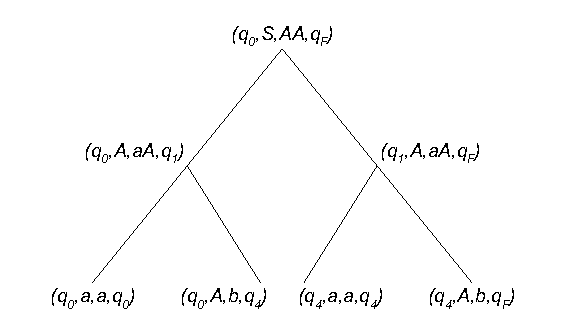
\includegraphics{img/gsystems/stromodv}
  \caption{Strom zodpovedajúci odvodeniu $S\Ra AA\Ra aAaA\Ra abab$}
  \label{gs_obr_stromodv}
\end{figure}

\begin{lema}
$TIME_{\mathcal{G}}(f(n))\subseteq 1NSPACE(f(n))$ pre $\forall
f(n)$.
\end{lema}

\begin{dokaz}
Nech $G=(N,T,M,\sigma)$ je $g$-systém pracujúci v čase $O(f(n))$.
Chceme skonštruovať Turingov stroj $A$ s jednosmernou vstupnou
páskou, ktorý bude simulovať $G$ v priestore $O(f(n))$. Uvažujme
slovo $w\in L(G)$ a jeho príslušný strom odvodenia $T$. Chceme
ukázať, že $A$ akceptuje $w$ práve vtedy, keď $w\in L(G)$.  $A$
bude na svojej pracovnej páske zapisovať cesty z $T$ vedúce od
koreňa k listom (obr.\ref{gs_obr_nspace}). $A$ bude hádať tieto cesty a
overovať, či jednotlivé štvorice na rovnakej úrovni $T$ tvoria
výpočet 1-$a$-prekladača $M$ a či zreťazenie výstupov štvoríc v
listoch $T$ tvoria $w$.

\begin{figure}[!ht]
\centering
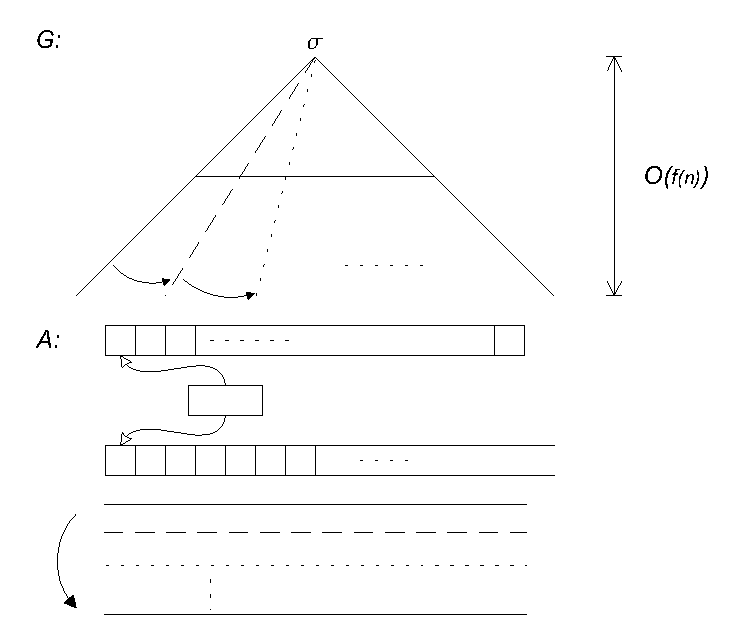
\includegraphics{img/gsystems/nspace}
\caption{Simulácia $g$-systému $G$ Turingovým strojom $A$}
\label{gs_obr_nspace}
\end{figure}

$A$ najprv uhádne a zapíše na pracovnú pásku cestu z koreňa do
najľavejšieho listu $\alpha$, pričom musí skontrolovať či prvá
štvorica je tvaru $(q_0,\sigma,u,q_F)$ a ostatné štvorice musia
začinať v stave $q_0$ a prepisovať prvý symbol výstupu
predchádzajúcej štvorice. Naviac výstup listu $\alpha$ musí byť
prefixom slova $w$. Ak nejaká z týchto podmienok neplatí, tak $A$
neuhádol najľavejšiu cestu správne a zasekne sa. Ak $A$ uhádol,
tak nahradí štvoricu $\alpha$ jeho najľavejším bratom $\beta$ (to
samozrejme tiež uhádne (obr.\ref{gs_obr_nstrom}a) a zaznačí si, že
$\beta$ je druhým synom ich spoločného otca $\gamma$. $A$ overí,
či $\beta$ je dobre uhádnutý t.j. počiatočný stav $\beta$ je
rovnaký ako koncový stav $\alpha$,  $\beta$ prepisuje druhý symbol
výstupu $\gamma$ a výstup $\beta$ je rovnaký ako ďalšia časť $w$
(bez prefixu, ktorý bol vo výstupe $\alpha$). Takto $A$ pokračuje
až kým neuhádne a neoverí posledného syna $\gamma$. Potom $A$
nahradí $\gamma$ jeho najľavejším bratom $\delta$ (podobne ako bol
$\alpha$ nahradený $\beta$). Teda $A$ robí prehľadávanie do hĺbky,
pričom si treba uvedomiť, že pri návrate na vyššiu úroveň v
strome, si $A$ musí pamätať koncové stavy jednotlivých vrcholov,
aby mohol pri hádaní ďalších vrcholov overiť správnu následnosť.

\begin{figure}[!ht]
\centering
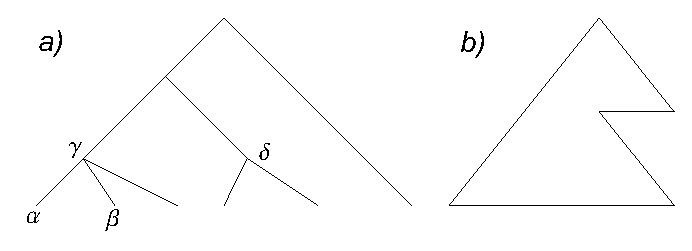
\includegraphics{img/gsystems/nstrom}
\caption{Nahrádzanie hrán v 1-$a$-prekladači $M$} \label{gs_obr_nstrom}
\end{figure}

Týmto spôsobom $A$ pokračuje až kým vo výstupoch listov nenájde
celé slovo $w$. Potom už $A$ vie, že všetky ostatné neoverené
listy musia mať na výstupe $\varepsilon$ (obr.\ref{gs_obr_nstrom}b). Teda
zvyšné cesty bude $A$ hľadať s tým, že v listoch musí byť na
výstupe $\varepsilon$. Keď $A$ dosiahol najpravejší list (to je,
ako inak, opäť uhádnuté), tak $A$ overí či všetky koncové stavy vo
všetkých štvoriciach na celej pracovnej páske sú $q_F$. Ak je to
tak, potom $A$ akceptuje $w$.

Z konštrukcie $A$ je zrejmé, že $A$ akceptuje $w$ práve vtedy, keď
$w\in L(G)$. Keďže $w\in L(G)$, tak hĺbka stromu odvodenia nie je
väčšia ako $c.f(|w|)$ kde $c$ je konštanta nezávislá od $w$, teda
hĺbka stromu odvodenia je $O(f(n))$, a teda $A$ na akceptovanie
slova $w$ nepotrebuje viac políčok na páske ako $O(f(n))$ z čoho
konečne plynie, že $L(G)\in 1NSPACE(f(n))$.
\end{dokaz}

\begin{lema}
$1NSPACE(f(n))\subseteq TIME_{\mathcal{G}}(f(n))$ pre $f(n)=\Omega
(\log n)$.
\end{lema}

\begin{dokaz}
Nech $A$ je nedeterministický Turingov stroj s jednosmernou
vstupnou páskou, ktorý akceptuje v priestore $O(f(n))$. Bez ujmy
na všeobecnosti predpokladajme, že $A$ má len jednu jednosmerne
nekonečnú pracovnú pásku.

Očíslujme políčka pracovnej pásky 0,1,2\dots Chceme skonštruovať
$g$-systém $G$, ktorý simuluje $A$ v čase $O(f(n))$. Jedna vetná
forma $G$ obsahuje informáciu o políčku pracovnej pásky $A$ počas
celého výpočtu. Nasledujúca vetá forma obsahuje informáciu o
nasledujúcom políčku atď. Keďže $A$ pracuje na najviac $O(f(n))$
políčkach, tak $G$ potrebuje na vygenerovanie slova dĺžky $n$
najviac $O(f(n))$ vetných foriem (t.j. $G$ pracuje v čase
$O(f(n))$). Samozrejme $G$ musí zaručiť konzistentnosť medzi
jednotlivými políčkami pásky, stavmi $A$ a symbolmi na vstupnej
páske podľa $\delta$-funkcie $A$.

Uvažujme jeden výpočet $A$ na vstupnom slove $w\in L(A)$. Nech $s$
je priestor a $t$ je čas potrebný na výpočet $w$. Odvodenie slova
$w$ $g$-systémom $G$ je tvaru:

\centerline{$\sigma =w_0\overset{k}\Ra w_k\Ra w_k'\Ra w_{k+1}\Ra
w_{k+1}'\Ra\dots\Ra w_{k+s}\Ra w_{k+s}'\Ra w$} kde vetná forma
$w_{k+j}$ drží obsah $j$-teho a $j+1$. políčka $A$ v celom výpočte
$A(w)$ a vetná forma $w_{k+j}'$ je použitá na overenie či uhádnuté
obsahy sú legálne vzhľadom na $\delta$-funkciu $A$.\\ $i$-ty
symbol vetnej formy $w_{k+j}$ je päťposchodový symbol obsahujúci:

\begin{itemize}
  \item stav $p_i$, v ktorom je $A$ v čase $i$ ($p_{t+1}$ je akceptujúci)
  \item symbol $a_i$, ktorý v čase $i$ číta vstupná hlava $A$, pričom tento symbol si
  označíme, ak v čase $i$ $A$ posúva hlavu na vstupe
  \item symbol $b_{j,i}$, ktorý je na $j$-tom políčku pracovnej pásky $A$ v čase $i$
  \item symbol $b_{j+1,i}$, ktorý je na $j+1$. políčku pracovnej pásky $A$ v čase $i$
  \item špeciálny symbol $0$, ak hlava bola na $j$-tom políčku, špeciálny symbol $1$, ak
  hlava bola na $j+1$. políčku a v ostatných prípadoch špeciálny
  symbol -
\end{itemize}

V prvých $k$-krokoch $G$ odvodí (uhádne\footnote{to sa dá na
$O(f(|w|))$ krokov keďže $A$ pracuje v priestore $O(f(|w|))$ a
teda v čase $O(|w|.c^{f(|w|)})$ pre nejakú konštantu $c$ t.j.
počet všetkých možných konfigurácií $A$ pri výpočte $w$. $g$-systém vie toľkoto
symbolov vygenerovať v logaritmickom čase, čo je v tomto prípade $O(f|w|)$.}) vetnú
formu $w_k$ dĺžky $t+1$ t.j. postupnosť stavov, ktorými $A$
prechádza počas výpočtu na $w$, vstupné slovo a časy, v ktorých
$A$ pohne hlavou na vstupe, obsahy nultého a prvého políčka
pracovnej pásky $A$ počas celého výpočtu a časy výskytu hlavy na
nultom políčku pracovnej pásky. Schématicky vyzerá vetná forma ako
na obrázku \ref{gs_obr_time_g}.

\begin{figure}[!ht]
  \centering
  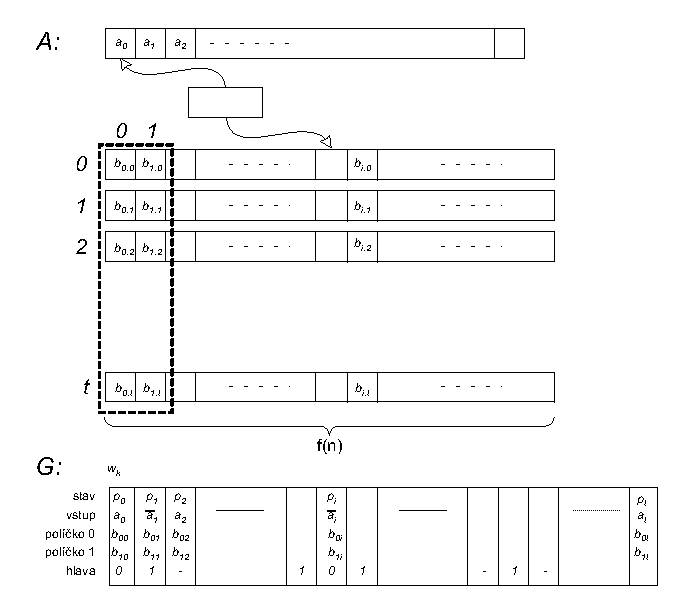
\includegraphics{img/gsystems/time_g}
  \caption{Simulácia TS $A$ $g$-systémom $G$} \label{gs_obr_time_g}
\end{figure}

V kroku $k+1$ $G$ overí či, to čo uhádol v predchádzajúcom kroku
je v súlade s $\delta$-funkciou $A$ a vygeneruje\footnote{tento
krok je naozaj iba overovací, to znamená, že ak $G$ uhádol dobre,
tak $w_k'=w_k$ inak sa $G$ zasekne} $w_k'$. Ak to bolo uhádnuté
dobre, tak $G$ vygeneruje $w_{k+1}$ t.j. prvé a druhé poschodie
bude rovnaké ako v $w_k'$, štvrté poschodie $w_k'$ bude vo
$w_{k+1}$ tretím poschodím, a kde bol v piatom poschodí $w_k'$
špeciálny symbol $1$, tam bude v piatom poschodí $w_{k+1}$
špeciálny symbol $0$, ostatné $G$ uhádne\footnote{t.j. $G$ uhádne
symboly na druhom políčku pracovnej pásky $A$ počas celého výpočtu
a časy výskytu hlavy na prvom políčku} (obr.\ref{gs_obr_time_g2}). V
ďalšom kroku $G$ overí či to čo uhádol teraz je legálne vzhľadom
na $\delta$-funkciu $A$ a vygeneruje $w_{k+1}'$\dots

Overovanie vo všeobecnosti vyzerá tak, že $G$ akoby sa naraz
pozeral na dva susedné päťposchodové symboly, takže vidí isté malé
okolie (2 symboly) pracovnej pásky v istom malom časovom úseku (2
takty TS) a k zmenám na pracovnej páske hľadá príslušnú časť
$\delta$-funkcie, ktorá je schopná takéto zmeny spôsobiť. Ak
takúto časť $\delta$-funkcie $A$ nájde, tak tieto dva
päťposchodové symboly môžu stáť vedľa seba a $G$ sa posunie o
jeden päťposchodový symbol. Takto môže $G$ overiť celú vetnú
formu.

$G$ pokračuje v striedaní hádacích a overovacích krokov, až kým
neodvodí vetnú formu bez špeciálnych symbolov výskytu hlavy na
pracovnej páske $A$ t.j. v piatom poschodí vetnej formy sa
nevyskytuje $0$ ani $1$. To znamená, že $G$ odsimuloval celý
výpočet $A$.

\begin{figure}[!ht]
  \centering
  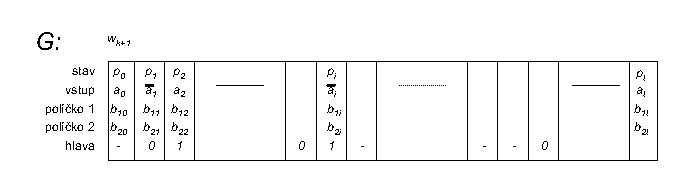
\includegraphics{img/gsystems/time_g2}
  \caption{Posun symbolov vo vetnej forme} \label{gs_obr_time_g2}
\end{figure}

V poslednom kroku $G$ prepíše vetnú formu tak, že každý
päťposchodoví symbol sa prepíše na symbol z druhého poschodia
(t.j. symbol zo vstupnej pásky $A$) ak bol tento symbol označený,
inak sa celý päťposchodový symbol prepíše na $\varepsilon$.

Zrejme $w\in L(G)\Longleftrightarrow$ ak $w$ je akceptované $A$.
Naviac $w$ je vygenerované v čase\newline
$O(f(n))+O(2f(n))=O(f(n))$. Samozrejme dva kroky odvodenia $G$
$w_l\Ra w_l'\Ra w_{l+1}$ sa dajú nahradiť jedným, potom $w$ je
vygenerované v čase $O(f(n))+O(f(n))=O(f(n))$. Tento spôsob
odvodenia sme zvolili iba pre lepšiu čitateľnosť dôkazu.
\end{dokaz}

\medskip
Predchádzajúce dve lemy nám umožňujú vysloviť nasledujúce tvrdenie:

\begin{veta}
$TIME_{\mathcal{G}}(f(n))=1NSPACE(f(n))$ pre $f(n)\geq\log n$.
\end{veta}

Ak si uvedomíme, že pre $f(n)\geq n$ je pracovná páska Turingovho
stroja dosť dlhá, aby sme si na nej zapamätali vstup, potom
$1NSPACE(f(n))=NSPACE(f(n))$.

Ďalším jednoduchým pozorovaním zistíme, že ak $f(n)\geq n$, tak
priestor na $TS$ a na $g$-systémoch je ekvivalentný, teda
$NSPACE(f(n))=SPACE_{\mathcal{G}}(f(n))$.

Môžeme teda vysloviť nasledovné dôsledky predchádzajúcej vety:

\begin{dosledok}
$TIME_{\mathcal{G}}(f(n))=NSPACE(f(n))$ pre $f(n)\geq n$.
\end{dosledok}

\begin{dosledok}
$TIME_{\mathcal{G}}(f(n))=SPACE_{\mathcal{G}}(f(n))$ pre $f(n)\geq
n$.
\end{dosledok}

\pagebreak

\section{Niektoré vlastnosti ``rýchlo generovateľných'' jazykov}

``Rýchlo generovateľné'' jazyky nazývame také jazyky z triedy
$TIME_{\mathcal{G}}(f(n))$, pre ktoré $f(n)<n$.

\begin{veta}
$TIME_{\mathcal{G}}(\log^p n)$ je $\mathcal{AFL}$
pre\footnote{rýchlejšie ako v logaritmickom čase $g$-systém
nedokáže pracovať} $p\geq 1$.
\end{veta}

\begin{veta}
$TIME_{\mathcal{G}}(\log^p n)\subsetneq TIME_{\mathcal{G}}(\log^q
n)$ pre $q>p>1$.
\end{veta}

\begin{dosledok}
Hierarchia $TIME_{\mathcal{G}}(\log^p n)$ pre $p>1$ je nekonečná.
\end{dosledok}

\begin{veta}
Pre každý jazyk $L\in\mathcal{L}_{RE}$ existuje $L'\in
TIME_{\mathcal{G}}(\log n)$ a existuje homomorfizmus $h$ taký, že
$L=h(L')$.
\end{veta}

\begin{dokaz}
Táto veta nám hovorí, že ku každému jazyku $L\in\mathcal{L}_{RE}$
vieme nájsť $g$-systém $G$ pracujúci v logaritmickom čase a
homomorfizmus $h$ taký, že $h(L(G))=L$. Veta \ref{gs_veta_gre} nám
hovorí, že vieme k $L$ nájsť príslušný $g$-systém $G$, ale
nezaručuje, že bude pracovať v logaritmickom čase. $G$ upravíme na
$G'$ nasledovne:
\begin{itemize}
\item Do 1-$a$-prekladača $G$ zavedieme nový terminál $\gamma$
\item Každú štvoricu tvaru $(q_0,\sigma ,u,p)$ nahradíme štvoricou $(q_0,\sigma ,\gamma u,p)$
\item Pridáme štvoricu $(q_0,\gamma,\gamma\gamma,q_0)$
\end{itemize}
Ľahko vidno, že takto upravený $g$-systém $G'$ generuje jazyk

\centerline{$L'=\{\gamma^{2^m} w\mm w\in L(G)$ a $m$ je počet
krokov odvodenia $w$ v $G\}$} Zamyslime sa teraz nad časovou
zložitosťou $G'$. Zoberme si nejaké slovo $u=w{\gamma}^{2^k}\in
L'$ pre nejaké $k$. Zrejme $|u|\geq 2^k$, ale $G'$ toto slovo
vygeneruje v $k$ krokoch, teda v logaritmickom čase, a teda $L'\in
TIME_{\mathcal{G}}(\log n)$. Homomorfizmus $h$ zvolíme takto:
\begin{itemize}
\item $\forall a\in T: h(a)=a$
\item $h(\gamma)=\varepsilon$
\end{itemize}
To znamená, že $h$ vymaže všetky $\gamma$ zo slov $w\in L'$, ktoré
sme zaviedli $g$-systémom $G'$. Teda $h(L')=L$. Ak sa nad touto
konštrukciou ešte raz zamyslíme, zistíme, že my sme $g$-systém
nejakým spôsobom ``nezrýchľovali'', ale to, že sme jazyk dostali
do logaritmickej časovej zložitosti sme dosiahli tým, že dĺžku
slov z tohto jazyka sme natoľko zväčšili, že pri zachovaní počtu
krokov odvodenia bude tento jazyk vygenerovaný v logaritmickom
čase vzhľadom na túto zväčšenú dĺžku slova.
\end{dokaz}

\begin{dosledok}
Trieda $TIME_{G}(f(n))$ nie je uzavretá na ľubovoľný
homomorfizmus.
\end{dosledok}

\section{Záverom o $g$-systémoch}

Je vhodné si uvedomiť niekoľko významných faktov, ktoré nám model
generatívnych systémov priniesol.

Pre známe paralelné gramatiky, ktoré dokážeme simulovať na
$g$-systémoch, dostaneme priestorové ohraničenie najviac
$1NSPACE(f(n))$. Podobne, ak navrhneme nový paralelný model, ktorý
vieme ``tesne'' simulovať na $g$-systémoch, dostaneme priestorové
ohraničenie $1NSPACE(f(n))$. Naviac pre každý jazyk $L\in
1NSPACE(f(n))$ existuje nejaký typ paralelnej gramatiky, ktorá $L$
dokáže generovať v čase $f(n)$.
